\section{Reactor like TGE-model}\label{sec:thunderstorm/reactor}

% Gurevich2001.pdf -- рсчеты гуревича для неоднороного поля, добавить в раздел про реактор ~\cite{gurevich2001kinetic}
TODO(литобзор из статьи Егора)
Общим недостатком рассмотренных выше моделей является упрощенная модель электрического поля: оно считается однородным по величине и направлению, что очевидно не так и в полу должны присутствовать разного рода неоднородности, вызванные как краевыми эффектами, так и возникновением сложных конфигураций зарядов. Точное моделирование и анализ динамики лавин убегающих электронов представляет собой сложную задачу, поэтому рассмотрим упрощенную модель что бы оценить потенциальные результаты, которые могут принести исследования в данном направлении. 

Чем ситуация в неоднородном по направлению поле отличается от развития лавин в однородном поле? Когда поле однородно то если гамма-кванты рождают новые затравочные электроны, то лавины от этих электронов будут направлены в том же направлении что и  первая лавина, но при этом их вершина будет смещена к  краю облака, что будет постепенно приводить к затуханию (как показано в предыдущих главах). Если же поле неоднородно по направлению, то направление новых лавин зависит от локальной конфигурации поля и таким образом может возникнуть ситуация изображенная на рисунке --- гамма-кванты от первичной лавины "зажигают" новые локальные ускоряющие ячейки, которые генерирует гамма кванты с угловым распределение значительно развернутым относительно углового распределения исходной лавины, что способствует более равномерному распределению новых затравочных электронов по облаку и как следствие  самоподдерживающей генерации лавин убегающих электронов.
Что бы смоделировать этот процесс, мы рассмотрим такую модель:
\begin{itemize}
    \item Используем только один изменяемый параметр --- локальный коэффициент размножения гамма-квантов, который дает обобщенное описание состояние атмосферы (величины электрического поля, плотности воздуха, вероятности зажигания ячейки и. т. д.)
    \item  Пренебрежем значением энергии гамма-квантов, пробег гамма-квантов будем разыгрывать на основе экспоненциального распределения с фиксированной длинной свободного пробега, много меньшей размеров облака;
    \item Также мы будем считать что при взаимодействии он гарантированно зажигает ячейку (фактически вероятность зажечь ячейку мы спрятали в локальном коэффициенте размножения);
    \item При зажигании ячейки мы не моделируем прохождение электронной лавины, а сразу генерируем вторичные гамма-кванты, их количество разыгрывается с помощью распределения Пуассона с локальным коэффициентом размножения гамма-квантов в качестве среднего, направление движения рожденных гамма-квантов считается однонаправленным с направлением электрического поля в точке рождения;
    \item Электрическое поле генерируются случайным образом на основе положения электрических зарядов местоположения которых разыграны на основе гауссова случайного блуждания;
    \item Облако представляется в виде куба со стороной в один километр, частицы покинувшие облако перестают отслеживаться.
\end{itemize}

В результате моделирования можно выделить три сценария: 
\begin{itemize}
    \item При малых значения локального коэффициента размножения роста гамма-квантов не происходит и высокоэнергетические процессы быстро затухают;
    \item При локальном коэффициенте размножения равным примерно 1.7 становится возможным медленное нарастание числа гамма-квантов, которое приводит к относительно стабильному самоподдерживающийся процессу, который однако с течением времени все же затухает. В целом этот сценарий хорошо описывает TGE-подобные явления;
    \item При превышении локальным коэффициентом размножения значения 1.8 происходит взрывной экспоненциальный рост числа гамма-квантов. Быстрый рост и большое количество гамма-квантов позволяет сказать что этот сценарий хорошо описывают TGF-подобные явления.
\end{itemize}

Для того чтобы проиллюстрировать эти три сценария, в работе приведены графики роста числа гамма-квантов в облаке от времени. Так график показывает затухание процессов при недостаточном значении локального коэффициента размножения, в данном примере несмотря на то что начальные гамма-кванты смогли сгенерировать некоторое количество вторичных частиц за время порядка 300 микросекунд все процессы затухли. График напротив показывает экспоненциальный рост за времена порядка 50-100 микросекунд (следует отметить что это согласуется со временем реально наблюдаемых TGF) при значения локального коэффициента размножения большего 1.8. Очень интересен график в нем наблюдается постепенный рост на достаточно большом (порядка 3 секунд) времени, что позволяет нам перейти от действующий на микровременных масштабах TGF к долговременным TGE. 

\begin{figure}
    \centering
    \begin{overpic}[scale=.5]{thunderstorm/rltge/electric_streams.pdf}
        \put(15,53){\includegraphics[scale=.015]{thunderstorm/rltge/cell.pdf}}
        \put(20,69){\text{Ускоряющая ячейка}}
        \put(10,10){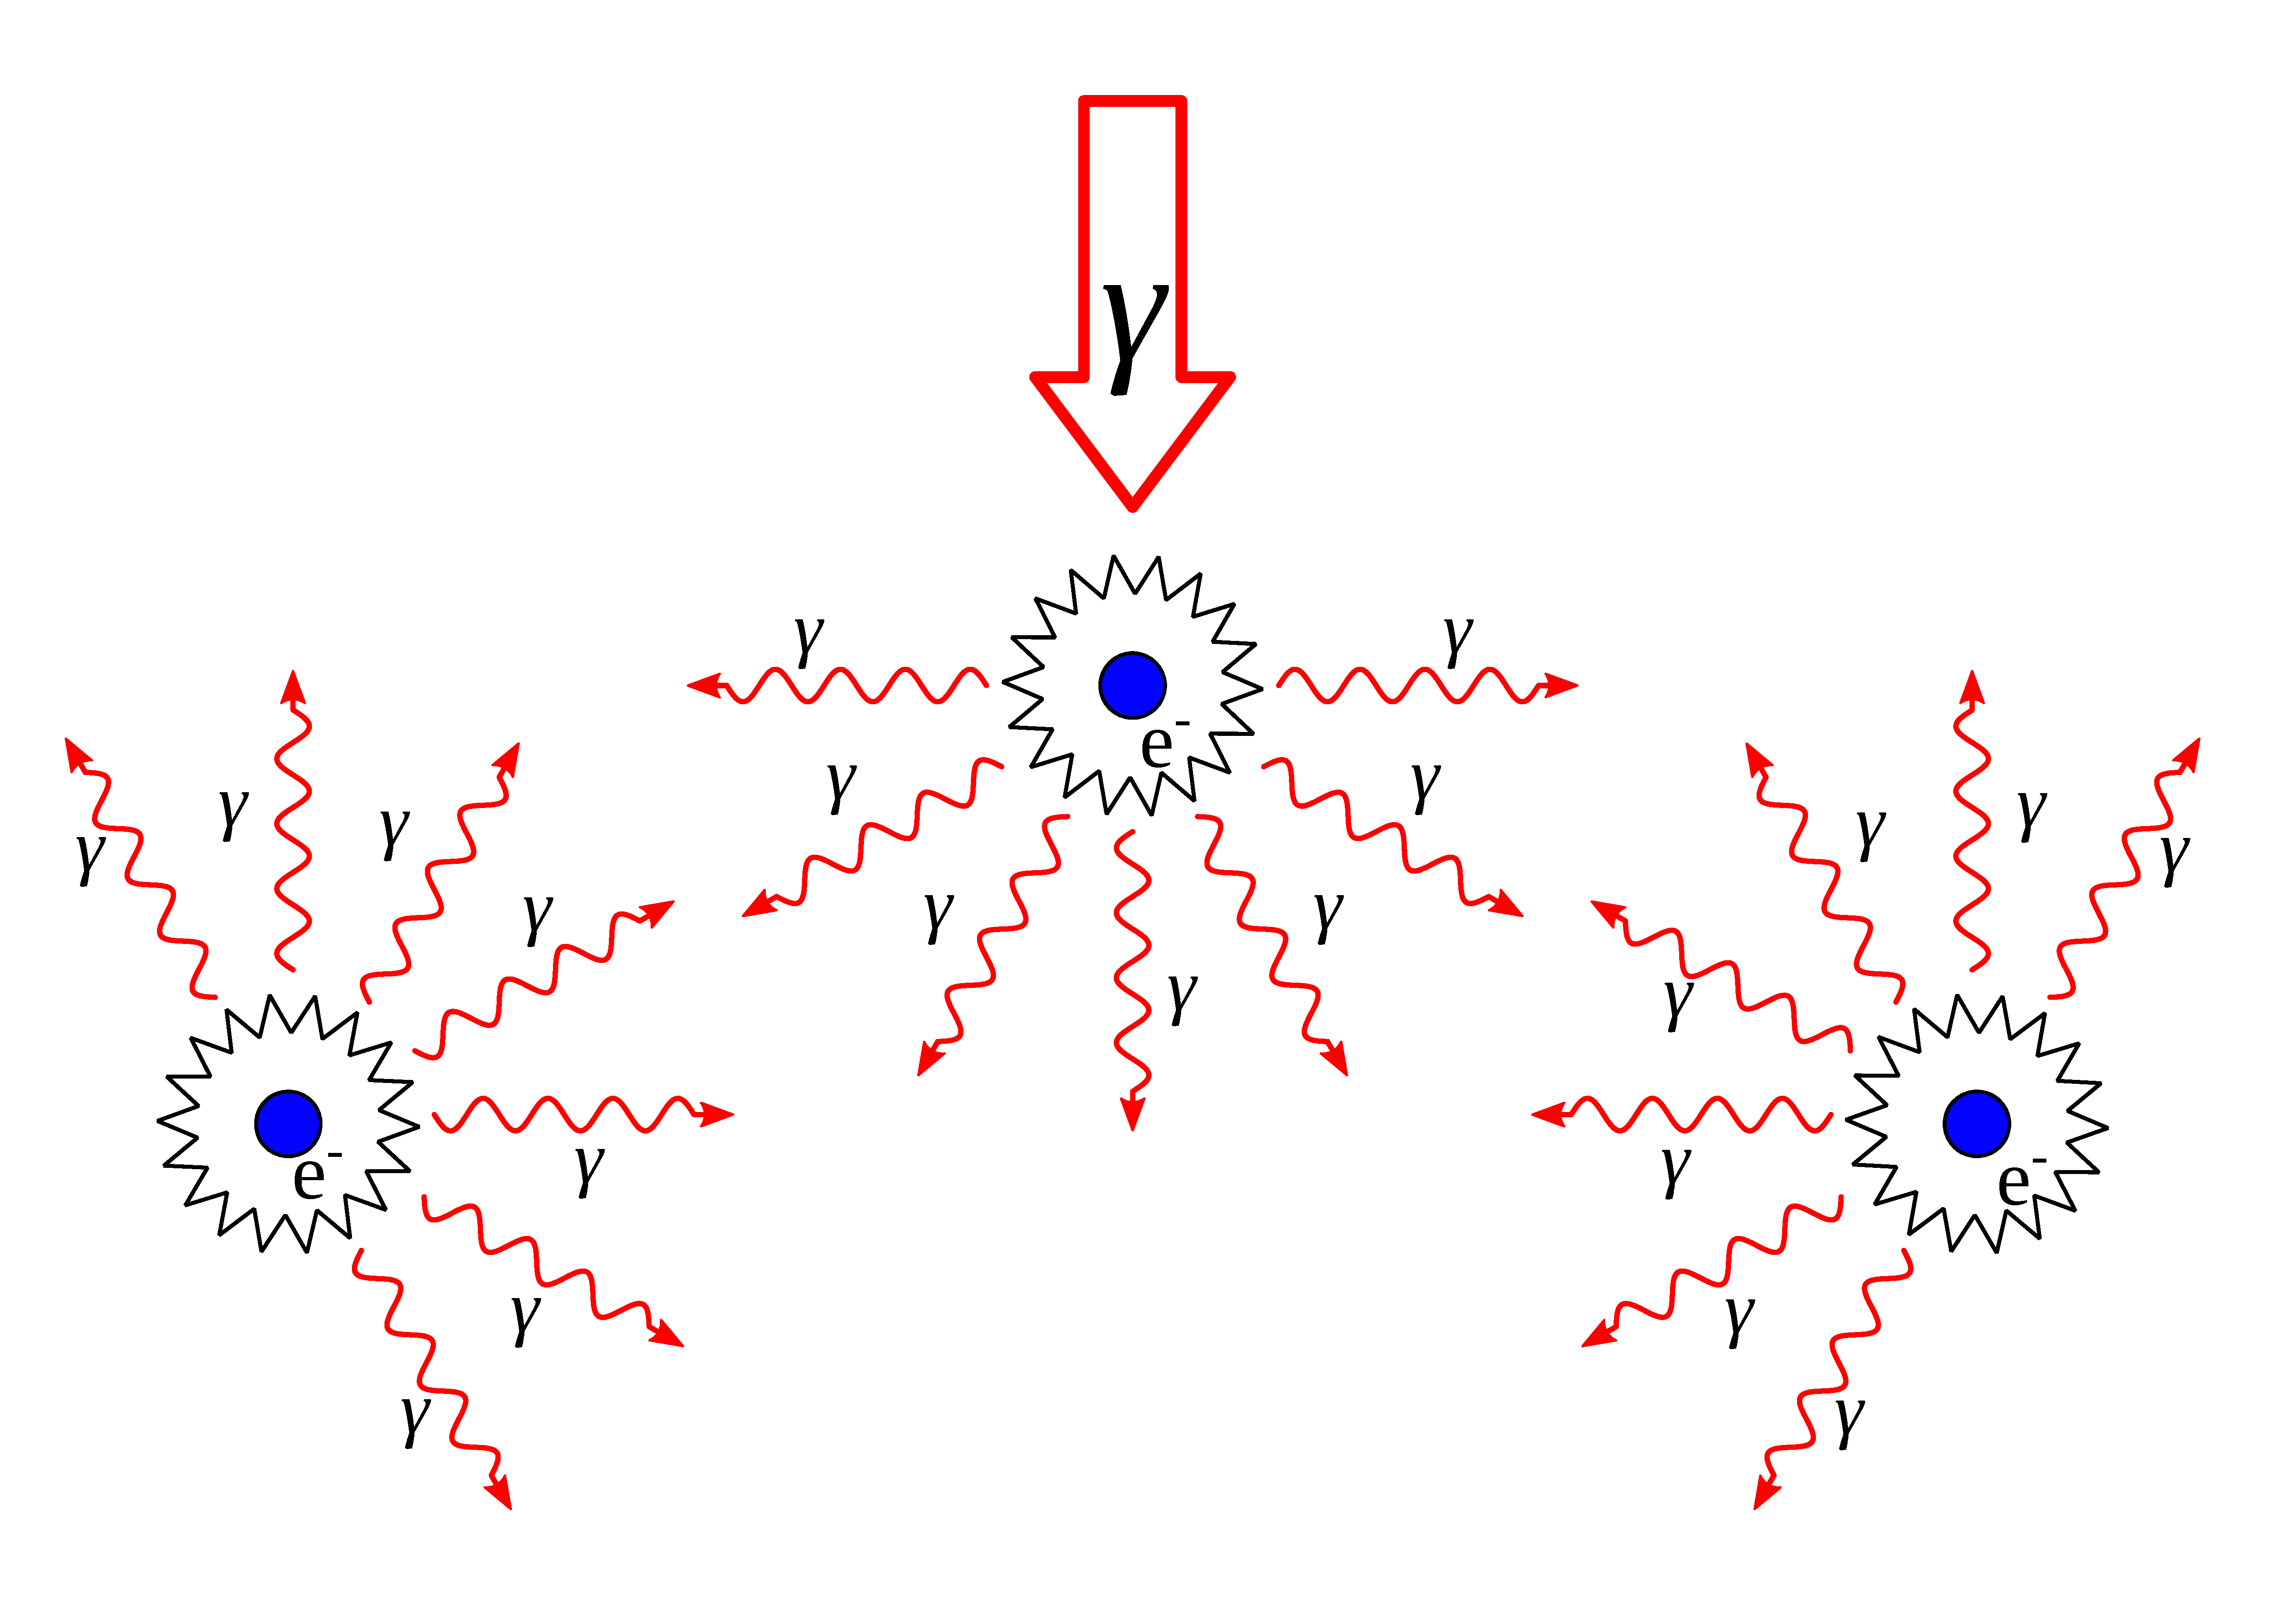
\includegraphics[scale=.15]{thunderstorm/rltge/draw.pdf}}
    \end{overpic}
    \caption{
        Processes occurring in the RL-TGE model: gamma quanta run local acceleration processes in different parts of the cloud with a multidirectional electric field.
    }
    \label{fig:rl}
\end{figure}


\begin{figure}[t]
    \begin{center}
        \begin{minipage}[h]{0.49\linewidth}
            \center{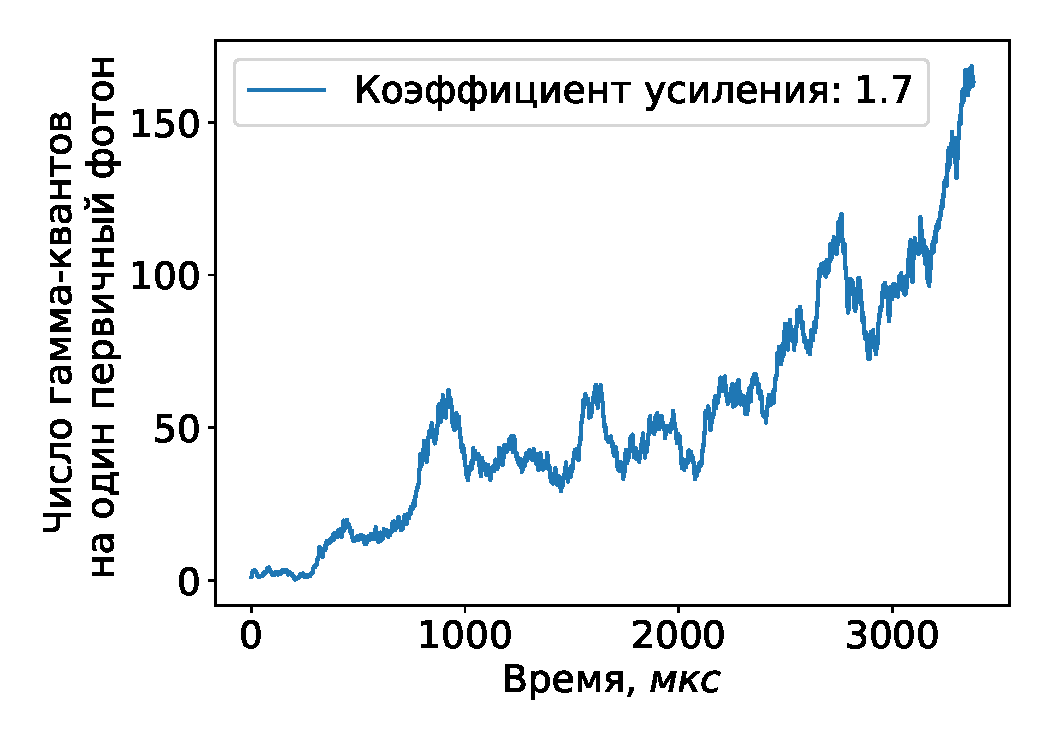
\includegraphics[width=\linewidth]{thunderstorm/RL_proofTGE.pdf} \\ а)}
        \end{minipage}
        \hfill
        \begin{minipage}[h]{0.49\linewidth}
            \center{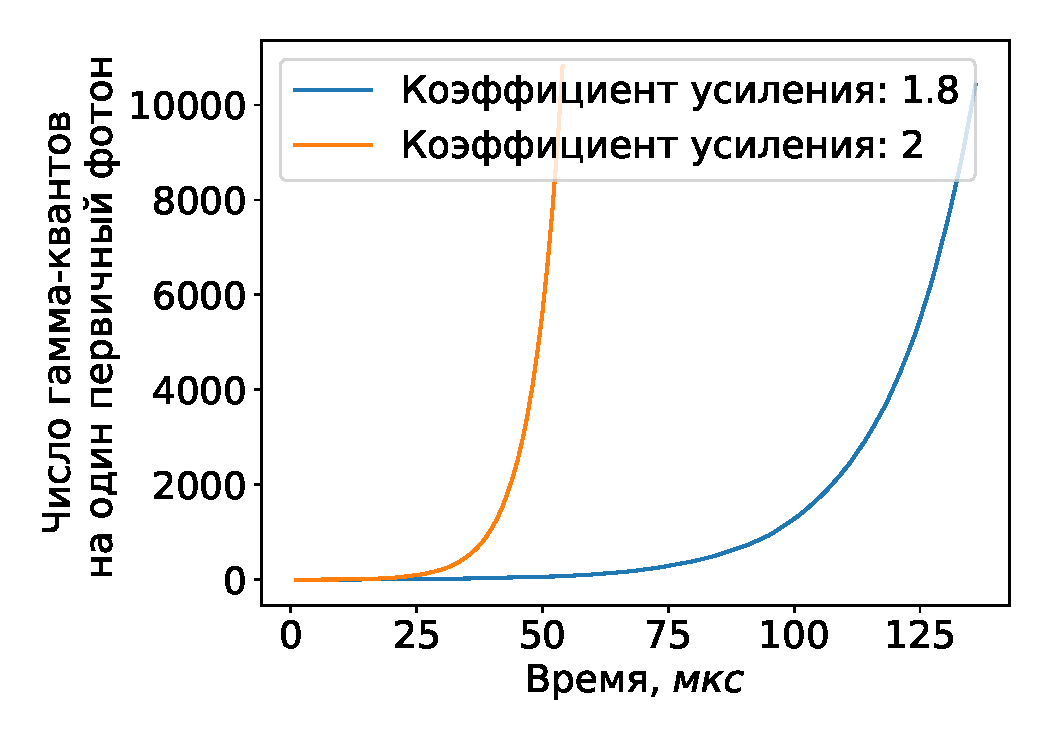
\includegraphics[width=\linewidth]{thunderstorm/RL_proofTGF.pdf}   \\ б)}
        \end{minipage}
        \caption{а) TGE-подобное нарастание. б) TGF-подобное нарастание.}
    \end{center}
    \label{thunder:rl_1}
\end{figure}


\begin{figure}[t]
    \begin{center}
        \begin{minipage}[h]{0.49\linewidth}
            \center{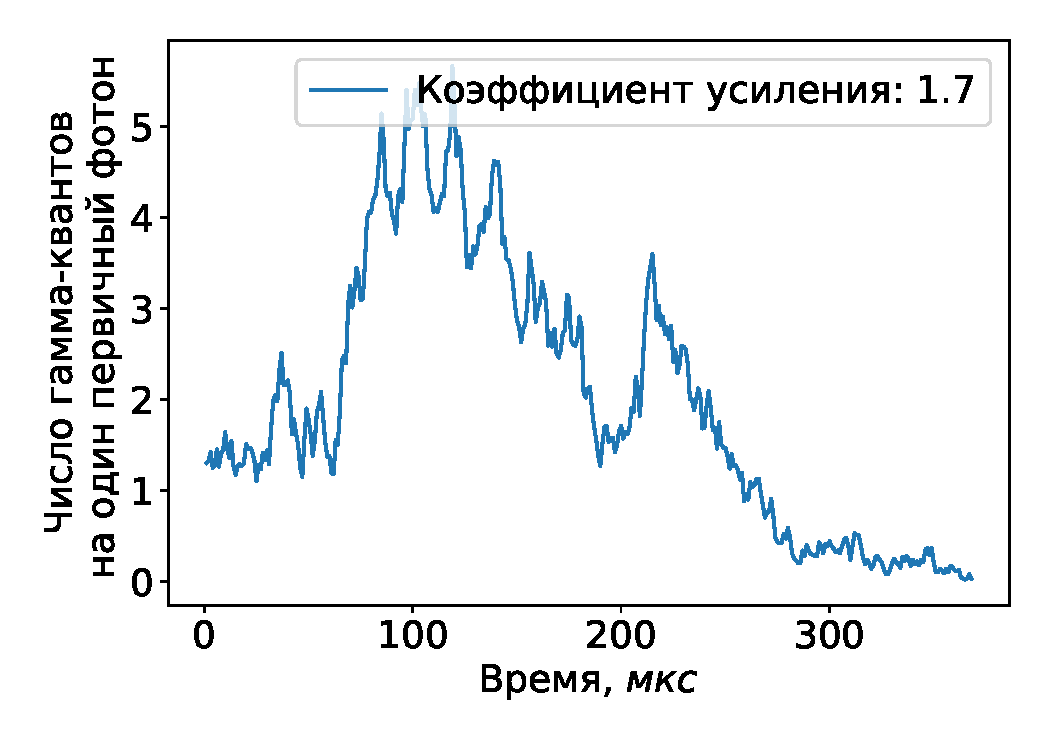
\includegraphics[width=\linewidth]{thunderstorm/RL_Extinction.pdf} \\ а)}
        \end{minipage}
        \hfill
        \begin{minipage}[h]{0.49\linewidth}
         %   \center{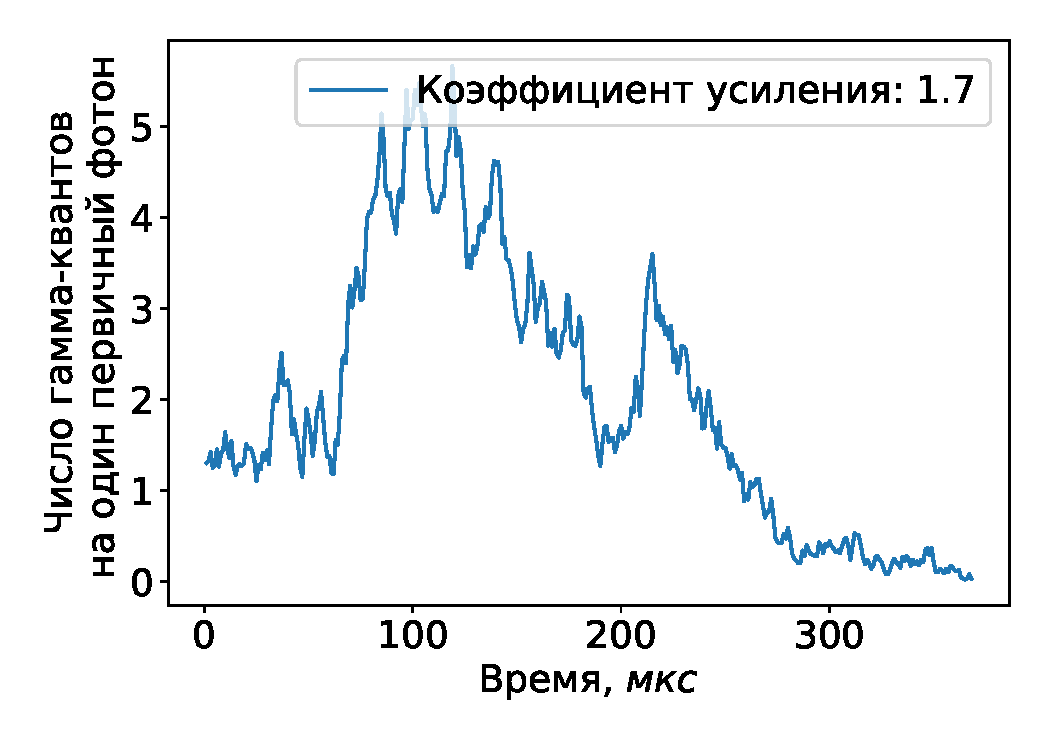
\includegraphics[width=\linewidth]{thunderstorm/RL_Extinction.pdf}   \\ б)}
        \end{minipage}
        \caption{а) Затухание лавины.}
    \end{center}
    \label{thunder:rl_2}
\end{figure}

Характер высокоэнергичных процессов в облаке в нашей модели напоминает происходящее в ядерных реакторах, где изменение одного параметра (коэффициента размножения нейтронов приводит либо к затуханию реактора, либо к стабильной выработке энергии, либо к взрыву топлива), поэтому мы называем нашу модель атмосферным реактором, и так же по аналогии можем выделить подкритический и критический режим работы реактора. Критический режим соответствует активному размножению гамма-квантов, которые порождают все больше лавин убегающих электронов что приводит к активной ионизации объема облака. Подкритический режим соответствует значению коэффициента размножения  при котором с одной стороны процессы в облаке постоянно стартуют в следствии подпитки внешними КЛ и затухают в следствии малости коэффициента размножения, с другой стороны  близкому к достаточному для начала работы в критическом режиме. Как показывает наше моделирование небольшое изменение локального коэффициента размножения позволяет перейти из подкритического режима в критический, что открывает для нас интересные возможности. Так облако можно представить как саморегулирующуюся системы в которой в следствии накопления заряда и роста электрического поля растет коэффициент размножения, что приводит к росту ионизации, что может приводить к появлению микроразрядов на гидрометеорах, что уменьшает коэффициент размножения и препятствует дальнейшей разрядке облака. Или например можно описать столкновение двух облаков, которые будучи в подкритическом режиме при столкновении переходят в критический режим. В целом проведенное моделирование хоть и носит очень приближенный характер, дает нам представление о перспективах модели со сложным полем по сравнению с более простыми моделями в которых рассматривается только однородное поле. Реакторная модель позволяет описывать рождение TGF и TGE в зависимости от состояние в облаке, внутриреакторные потоки гамма-квантов позволяют описать избыток нейтронов наблюдающийся в работе~\cite{gurevich2012strong}. Результаты моделирования изложен в работе~\cite{reactor}, исходный код доступен по ссылке.



\section{Анализ структуры грозового облака на основе наблюдения TGE}\label{sec:thunderstorm/llletge} 
В отличии от TGF представляющие собой очень короткие (~10 мкс) вспышки гамма- и рентгеновского излучения из грозового облака, TGE представляет собой длительное повышение гамма-фона. По результатам наблюдений на горе Арагац академиком Чилингаряном~\cite{PhysRevD.98.082001} была предложено разделить TGE на две условные группы: High Energy Particle TGE (HEP TGE) имеющие длительность порядка нескольких минут и значительную высокоэнергичную (энергия гамма-квантов более 3 МэВ) компоненту и Long-Lasting Low Energy TGE (LLLL TGE) имеющие длительность более двух часов и при этом содержащие в основном низкоэнергитичные (менее 3 МэВ) гамма-кванты. При этом можно отметить следующие особенности: 
\begin{itemize}
    \item HEP TGE  возникает при глубоких  провалах  приповерхностного поля, но не каждый провал сопровождается HEP TGE,
    \item Возможно существование LLLE TGE без  HEP TGE,
    \item Возможно существование LLLE TGE при полях ниже поля убегания электронов,
    \item HEP TGE может возникать несколько раз: оно может быть разрушено из-за вспышки молнии и потом восстановится.
\end{itemize}
В контексте изучения возникновения молнии HEP TGE и LLLE TGE интересны, так как они могут помочь описать структуру грозового облака.  Так первым представление об грозовом облаке был вертикальный диполь, однако реальная его структура гораздо сложнее, в данной работе мы рассмотрим генерацию TGE c точки зрения трипольной модели(хотя по всей видимости облака могут иметь и большее число слоев). При представлении облака как вертикального триполя считается что в центре облака собирается отрицательный заряд, в верхней части облака и на земле индуцируется положительный заряд, и наконец в нижней части облака формируется небольшая область с положительным зарядом. Тогда можно сформулировать следующие гипотезы:
\begin{itemize}
    \item Затравочными частицами служат электроны от космических лучей;
    \item LLLE TGE -возникает за счет поля между основным отрицательным зарядом и зарядом индуцированным в земле;
    \item По мере развития нижнего положительного заряда (НПЗ)  возрастает поле и поток частиц в LLLE TGE переходит в HEP TGE;
    \item Регистрация HEP TGE происходит при прохождении НПЗ над детектором
\end{itemize}
Для проверки этих гипотез в работе были проанализированны экспериментальные наблюдения которые сравнивались с моделированием с помошью CORSIKA и GEANT4. Далее приводятся результаты проведенного для работы~\cite{PhysRevD.98.082001}  автором диссертации GEANT4 моделирования. В частности автором были проведенным моделирования превышения гамма-квантов в зависимости от электрического поля, а также получены их угловые и радиальные распределения. Симуляция проводилась при следующих параметрах: первичными частиц являются гамма-кванты в диапазоне энергий от 1 до 100 МэВ, имеющие степенной спектр вида $E^{-1.42}$, начальная точка расположена в тысяче метрах над станцией(которая находится на высоте 3200 метров над уровнем моря), моделирование проводилось в подкритических полях (значение критического поля для данных высот порядка 1.7-1.8 кВ/см
), также моделирование проводилось с использование двух физических листов \textit{G4EmPhysStandard} и \textit{G4EmPhysStandard\_opt4} (использовался GEANT4 версии 4.10.4). TODO(График) График демонстрирует рост потока гамма-квантов, даже в подкритических полях и взрывной рост при приближении к порогу. Левый график демонстрирует радиальное расхождение гамма-квантов от RREA вследствии комптон-эффекта, как мы видим маловероятно наблюдать гамма-кванты на расстоянии большем километра от центра лавины, кроме того для гамма-квантов рассеявшихся на расстояние более километра, максимум по углу смещен в горизонтальный сторону, что затрудняет их регистрацию. Результаты моделирования автора согласуются с другим моделированием проведенным в программе CORSIKA, и на основе анализа приведенного в работе~\cite{PhysRevD.98.082001} можно утверждать что сформулированные гипотезы выполняются и можно сделать вывод что наблюдаемые данные по TGE могут быть объяснены трипольной структурой облака поля и наблюдение за TGE можно использовать для наблюдения эволюции нижнего заряженного слоя, его образования, перемещения и разрушения.

\section{Нейтроны в грозовых облаках}\label{sec:thunderstorm/neutron} 

Ещё одним интересным следствием из феномена убегающих электронов является наличие нейтронного излучение из грозового облака. Действительно так энергиях гамма-квантов в явлениях TGF и TGE может достигать десятков мегаэлектрон-вольт то становится возможным прохождение фотоядерных реакций, генерирующих поток нейтронов. Это следствие находит экспериментальные наблюдения, например исследование на научной станции на Тянь-Шане сначала регистрировали понижение потока нейтронов по время грозовой активности ~\cite{antonova2009effect}, но в более поздней работе отмечают регистрацию значительного роста потока нейтронов~\cite{gurevich2012strong}. Также повышение потока нейтронов подтверждаются наблюдения на научной станции на г. Арагац и наблюдениями японских ученых~\cite{enoto2017photonuclear}. Есть определенные вопрос к источнику нейтронов, ряд исследователей полагаю что повышение потока нейтронов обусловлено не проходящими в облаке фотоядерным реакциями, а обусловлено другими источниками, например вымыванием радиоактивных элементов из почвы во время дождя и выходом радона, но исследования в работе TODO() опровергают эту гипотезу.


Принимая гипотезу о том что повышение потока нейтронов связанно с происходящими в облаке высокоэнергетическими процессами, можно предположить что регистрация нейтронов может дать информацию о величине потока и энергетических характеристиках гамма-квантов в грозовом облаке. Поэтому в рамках проектирования орбитального детектора для проекта ЧИБИС был поднят вопрос о целесообразности размещения на спутнике детектора нейтронов. Для ответа на этот вопрос было проведено моделирование чтоб оценить потенциальный поток нейтронов который можно было бы измерить на орбите. В симуляциях запускались гамма-кванты двух энергий  (15 и 100 МэВ) с высоты 15 километров, и рассчитывалось распределение рождения нейтронов по высоте, определялись характеристики рожденных частиц, так же моделировалось рождение нейтронов в детекторе из полистирола. 

\begin{figure}[t]
    \begin{center}
        \begin{minipage}[h]{0.49\linewidth}
            \center{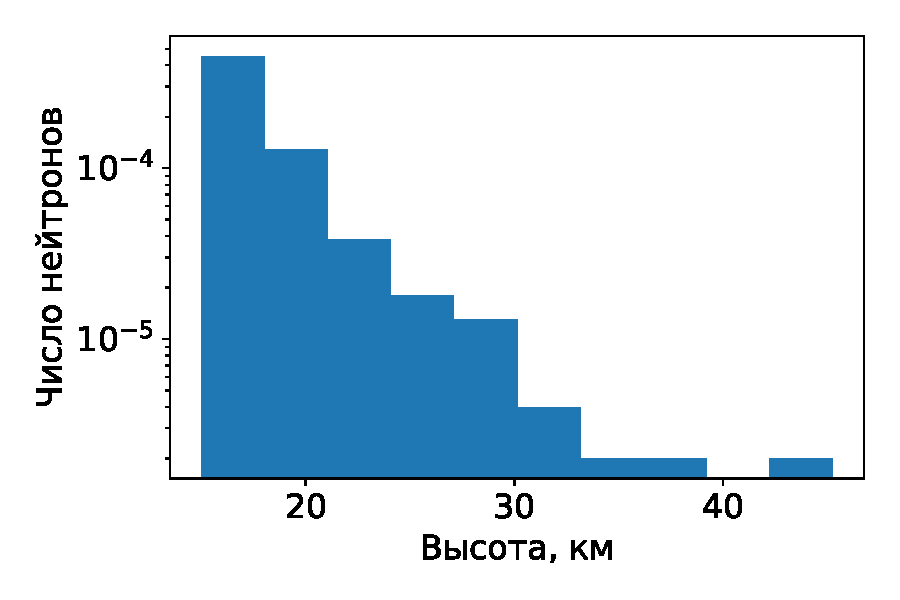
\includegraphics[width=\linewidth]{thunderstorm/neutron/air_z_15MeV.pdf} \\ а)}
        \end{minipage}
        \hfill
        \begin{minipage}[h]{0.49\linewidth}
            \center{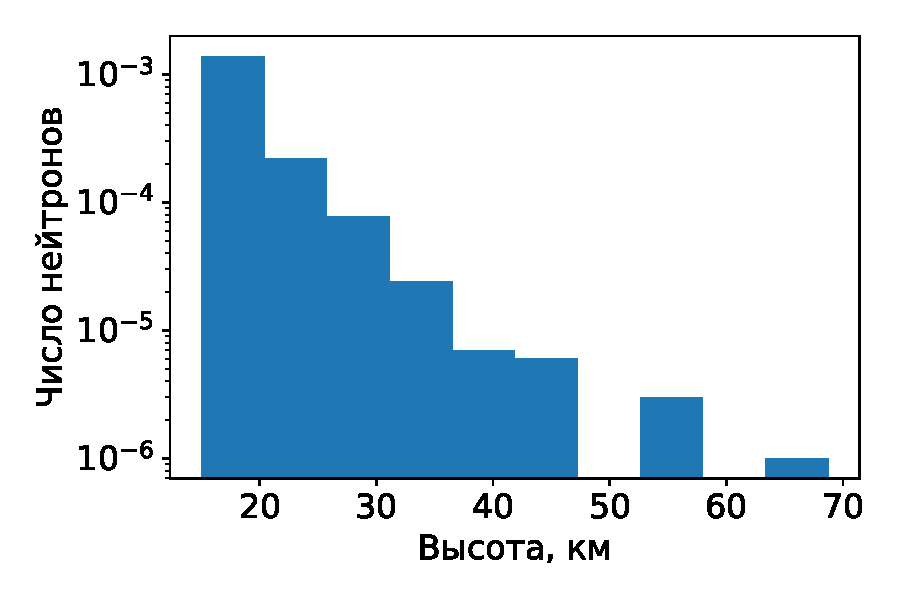
\includegraphics[width=\linewidth]{thunderstorm/neutron/air_z_100MeV.pdf}   \\ б)}
        \end{minipage}
        \caption{Распределение рождения нейтронов по высоте для фотонов с начальной энергией а) 15 МэВ б) 100 МэВ. Нормировано на одну первичную частицу.}
    \end{center}
    \label{fig:storm:neutron_z}
\end{figure}

По результатам моделирования для гамма-квантов с начальной энергией 100 МэВ получено что рождается примерно 1,7 на тысячу гамма-квантов с энергией 100 МэВ. Примерно половина нейтронов имеет энергию до 10 МэВ, вторая часть имеет медленно спадающий спектр в диапазоне от 10 до 70 МэВ. Разброс при рождении в атмосфере достаточно мал, порядка 85 \% нейтронов рождаются в стволе пучка гамма-квантов. Направление импульса рожденных нейтронов имеет достаточно широкий разброс, не позволяющий говорить о наличии выделенного направления движения. График~\ref{fig:storm:neutron_z}а показывает распределение точек рождение нейтронов по высоте. Как мы видим нейтроны рождаются на высотах до 70 километров, далее атмосфера становится сильно разреженной для того что бы шанс с рождения нейтрона был достаточно значительный. Можно отметить что в атмосфере взаимодействует только порядка 0.4 \% гамма-квантов, остальные 99.6\% улетают в космос. Также следует учесть то что гамма-кванты могут рождать нейтроны столкнувшись с корпусом космического аппарата (КА) и телом детектора, однако как показало моделирование, даже если считать что все долетевшие до КА частицы взаимодействуют в нем (что вообще говоря невозможно так как требует КА с массо-габаритным характеристикам значительно превосходящими реальные аппараты), то число таких нейтронов будет составлять только 8\% от числа рожденных в атмосфере.

Результаты моделирования для гамма-квантов с начальной энергией 15 МэВ в целом аналогичны, число рожденных нейтронов примерно в три раза меньше чем для 100 МэВ гаммы, они рождаются на высотах до 40 км (график распределения по высоте приведена на рис.~\ref{fig:storm:neutron_z}б). Только 5\% таких гамма-квантов долетает до космоса, и они не выбывают нейтроны с детектора в КА. Вопрос о достижимости детектора на КА рожденными в атмосфере нейтронов  является дискуссионным, простое GEANT4 моделирование показывает достаточно быструю потерю энергии быстрыми нейтронами, однако есть сомнения в точности выбранной модели, также есть работы показывающий что при больших потоков гамма-квантов возможно достижение нейтронами высот больших 400 км (ссылка а чувака). Однако те не менее моделирование показывает что число нейтронов будет не значительным и размещение детектора нейтронов на КА является не целесообразным и гораздо более эффективным является работа по  регистрации непосредственно гамма-квантов которые долетают до КА в больших количествах.
